\documentclass{article} % For LaTeX2e
\usepackage{nips13submit_e,times}
\usepackage{hyperref}
\usepackage{url}
\usepackage{graphicx}
\usepackage{amsmath}
\usepackage{amssymb}
%\documentstyle[nips13submit_09,times,art10]{article} % For LaTeX 2.09


\title{  Extracting Aspect-Level Sentiment from Product Reviews  }


\author{
Desmond C. Ong, Shane Soh, Matthew Long \\
Stanford University \\
\texttt{\{dco, shanesoh, mlong14\}@stanford.edu}
%Matthew Long \\
%Stanford University\\
%\texttt{mlong14} \\
%\And
%Desmond C. Ong \\
%%Psychology \\
%Stanford University \\
%\texttt{dco} \\
%\And
%Shane Soh \\
%%Affiliation \\
%Stanford University \\
%\texttt{shanesoh} \\
}

% The \author macro works with any number of authors. There are two commands
% used to separate the names and addresses of multiple authors: \And and \AND.
%
% Using \And between authors leaves it to \LaTeX{} to determine where to break
% the lines. Using \AND forces a linebreak at that point. So, if \LaTeX{}
% puts 3 of 4 authors names on the first line, and the last on the second
% line, try using \AND instead of \And before the third author name.

\newcommand{\fix}{\marginpar{FIX}}
\newcommand{\new}{\marginpar{NEW}}

\nipsfinalcopy % Uncomment for camera-ready version

\begin{document}


\maketitle

\begin{abstract}
Previous work in \textit{aspect-level sentiment analysis}---identifying the sentiment associated with various attributes of a product---have mostly been formulated as supervised learning problems, requiring labels of both the relevant aspects and their sentiment. Acquiring labels for sufficiently large datasets are however often costly and time consuming. Here we propose a largely unsupervised and scalable method for aspect-level sentiment analysis that consists of two steps: 1) discovery and extraction of aspects from product reviews via clustering of \texttt{word2vec} [i-ii] representations, 2) classifying aspect-specific sentiments using convolutional neural networks.
\end{abstract}

\section{Introduction}

In this day and age, consumers have unprecedented access to a deluge of information about products---most notably reviews written by other consumers---with which to make his or her purchase decisions. Unfortunately, sifting through hundreds of reviews across tens of different websites to acquire specific information about the product and its important attributes (e.g. \textit{battery life}, \textit{screen size}, or \textit{weight} in the case of electronic products) is a time-consuming chore. Aspect-level sentiment analysis would allow consumers to effortlessly compare general sentiments of various aspects of multiple similar products.

However, one of the biggest challenges in training aspect-specific sentiment analysis models is the lack of large datasets labeled with sentiment on the aspect-level (most datasets with sentiment labels existed on a document level). In this report, we propose a scalable method for extracting and classifying aspect-specific sentiments that is largely unsupervised. To do this, we tackle two separate but interconnected components of this problem: 1) discovery of aspects, and 2) aspect-specific sentiment classification.

Within the context of a product review, the first component, \textit{aspect discovery}, involves identifying individual ``aspects" (which could be the product itself, or features/attributes of the product). This is made more difficult by the fact that relevant aspects might differ greatly across products in the same category. For example, aspects revelant to a cellular phone might be \textit{battery life}, \textit{screen size}, \textit{weight} and \textit{cost}. Not all these aspects are relevant across electronic items: for instance, \textit{screen size} might be irrelevant for a pair of headphones or a video game controller. We tackle this problem by generating new aspects from a list of seed words based on cosine similarities of the \texttt{word2vec} representations [i-ii], and using the discovered aspects to train an aspect classifier.

The second component, \textit{aspect-specific sentiment classification} involves identifying the sentiment associated with each aspect [1-6]---\textit{very positive, positive neutral, negative or very negative}. We approach this problem by first using a lexicon-based heuristic as a baseline and as a means of \textit{pre-labeling} the data. We then refined the labels and trained a convolutional neural network [Yoon Kim] to tackle the sentiment analysis problem as a sentence classification problem.

\section{Related work}


\textbf{Aspect Discovery}: Previous methods have used graphical models to attempt to extract latent sentiment. [1-3] use Latent Dirichlet Allocation, while [4] uses a Conditional Random Field model to model latent aspects. In particular, most of these methods have a generative model where there is a latent aspect (drawn from a mix of ``global" and ``local" topics [1-2], or latent to each sentence [3]). 

% Add in "Simpler is better" paper

[aspect parser paper]: rule-based approach to extracting aspects

\textbf{Aspect-specific Sentiment Classification}: There has been recent work on using convolutional neural networks (CNN) trained on top of pre-trained word vectors for sentence-level classification tasks [Kim]. Specifically, [Kim] demonstrated the use of CNN to outperform state-of-the-art models on sentiment analysis classification tasks. Other deep learning approaches for aspect-based sentiment analysis use hierarchical models such as a Recursive Neural Tensor Network (RNTN) to extract aspect-sentiment tuples. Unfortunately, such supervised methods (e.g. [5-7]) that require labeled aspects-sentiment pairs for training are unscalable, and a better approach would be to automatically identify relevant aspects for each product (which, e.g. [1-3] try to do via topic modeling). 

% TODO: Desmond to add more references?

\section{Dataset}
The dataset that we used consists of 7.6 million reviews of electronic products from Amazon.com [8]. These reviews comprise 39.4 million sentences. Each review is only labeled with the document-level 5 star rating, which we did not end up using as it was too coarse. We focused our attention only on the raw natural language text, which is unlabeled.

\textbf{Preprocessing.} We tokenized our corpus using NLTK's punkt tokenizer [9] for sentence splitting. We then removed all non-alphanumerical characters and replaced all digits with \texttt{DG}. Finally, we performed collocation detection to detect common bigrams.

\section{Approach}

Our proposed workflow can be divided into two main parts: {\bf Aspect Discovery} and {\bf Aspect-Specific Sentiment Classification}. See Fig. \ref{workflow} for an illustration.

\begin{figure}[ht]
\begin{center}
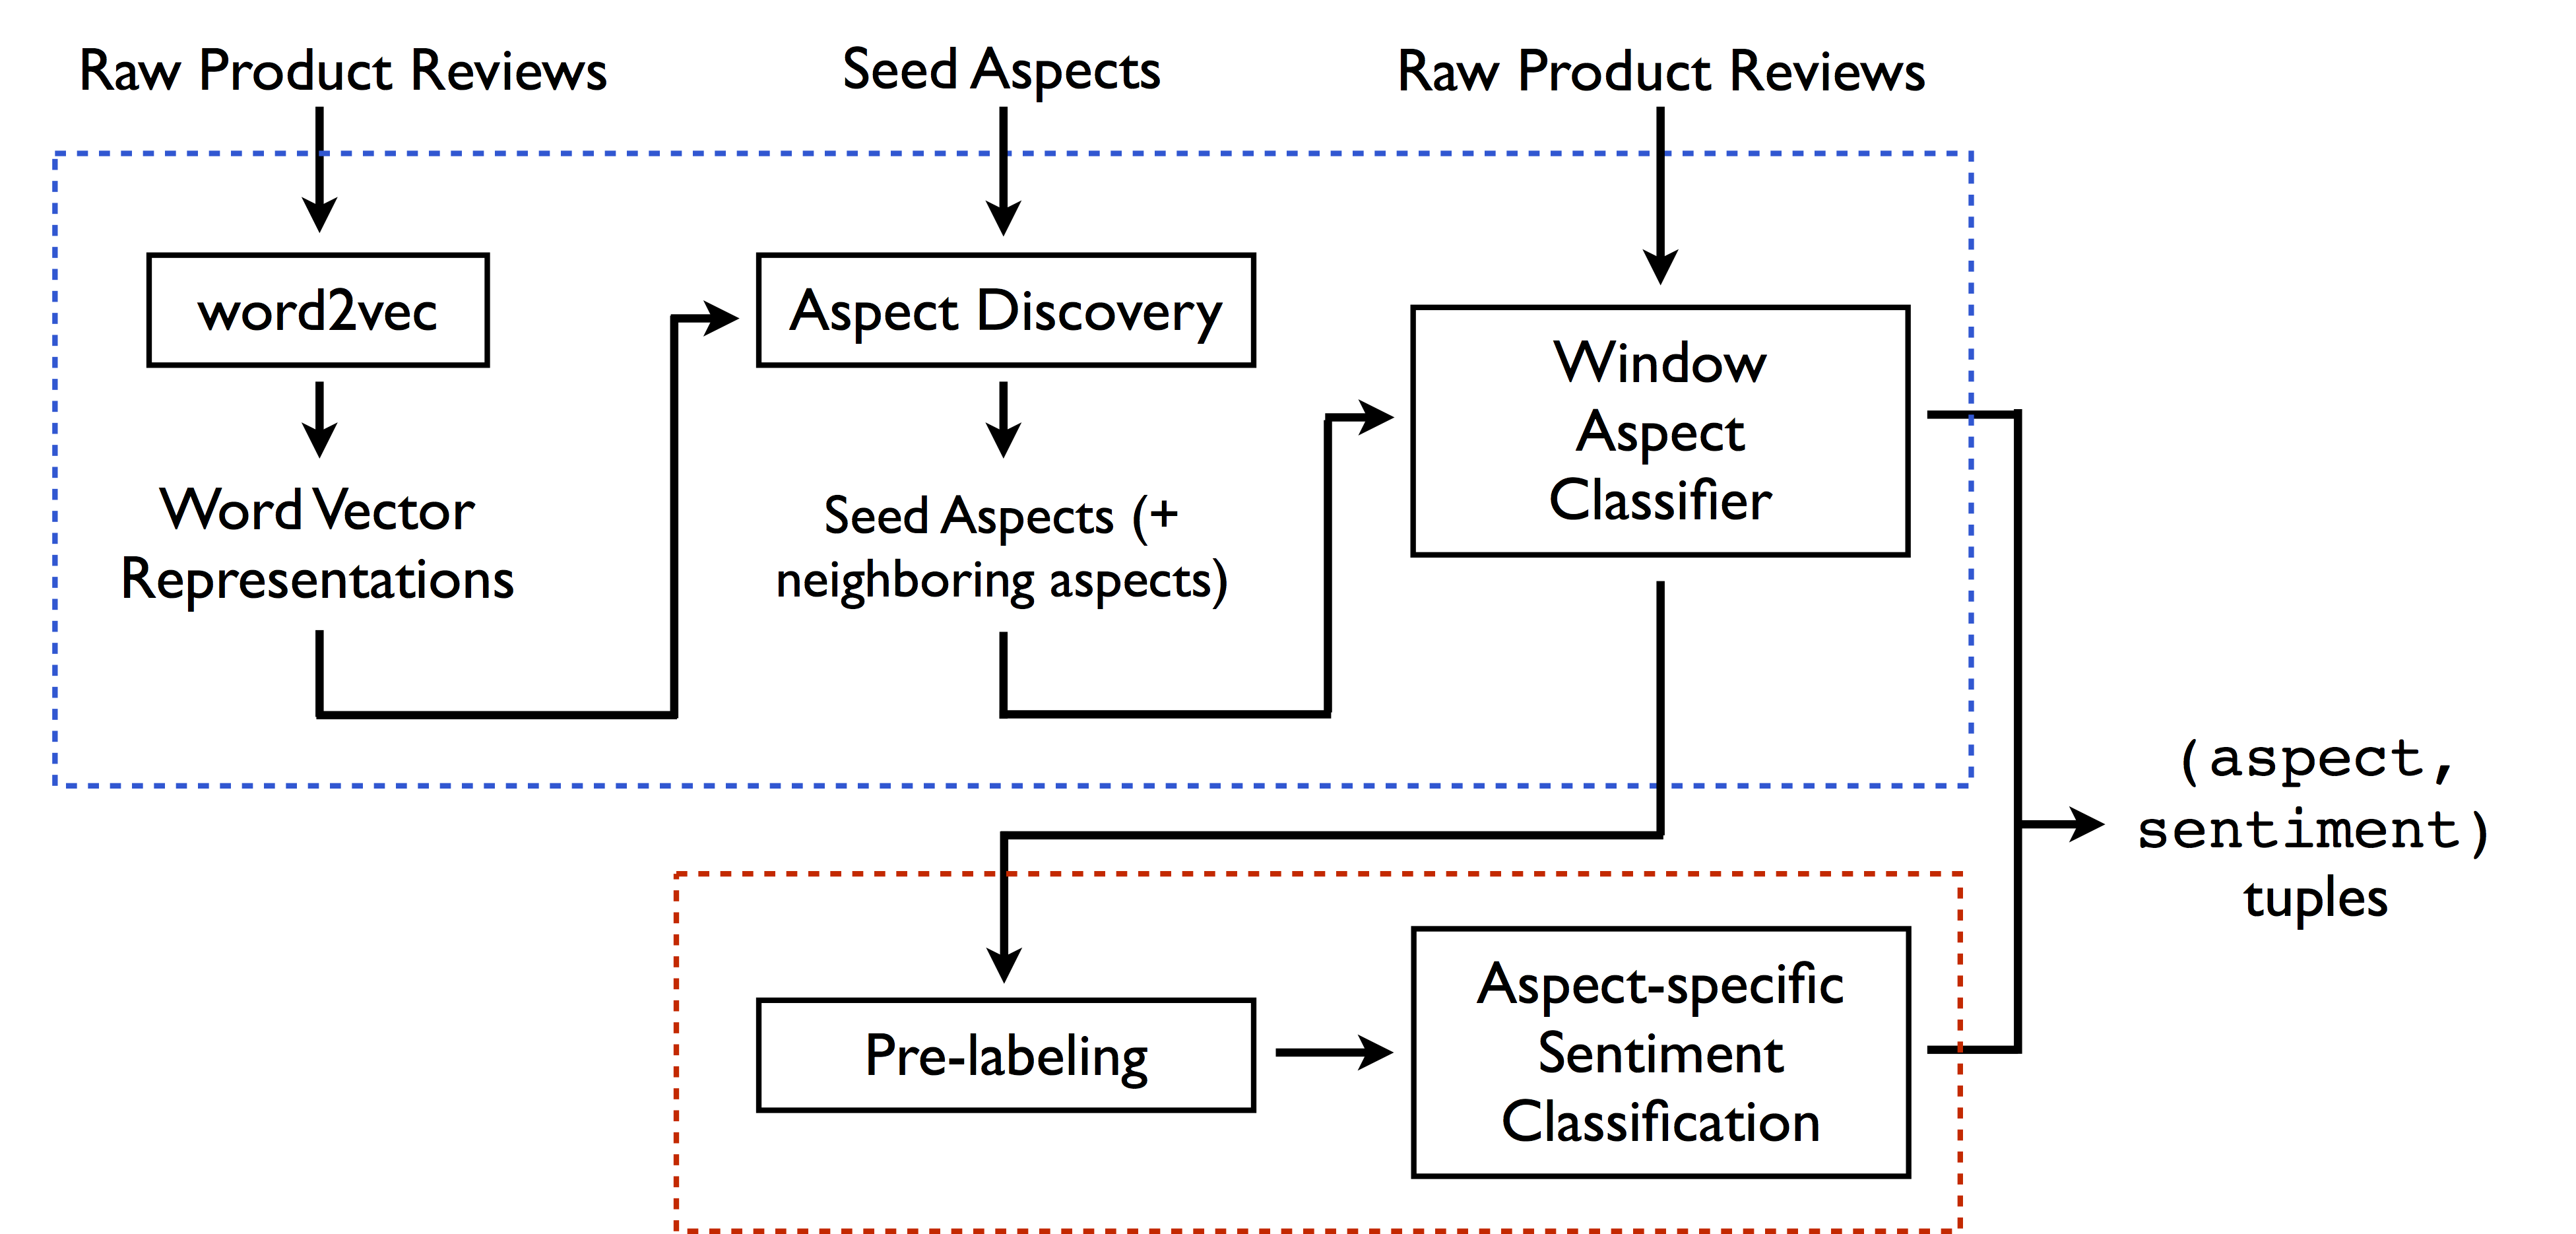
\includegraphics[width=.85\columnwidth]{workflow.png}
\end{center}
\caption{Proposed Workflow. We generate a list of seed aspects specific to the product category. We then discover neighboring aspects based on cosine distances to the seed aspects' \texttt{word2vec} representations. We then train a \textit{window aspect classifier} to discover more aspects from raw text. Next, we use a lexicon-based heuristic to \textit{pre-label} the expanded list of aspects which are subsequently refined by hand. Lastly, we train a supervised CNN to do the \textit{aspect-specific sentiment classification} to produce \texttt{(aspect, sentiment)} tuples.}
\label{workflow}
\end{figure}

\subsection{Aspect Discovery}

\subsubsection{Generating Seed Aspects}
The first part of our workflow involves generating a list of seed aspects. These seed aspects do not require domain-specific knowledge and can be fairly general (the idea is that any layperson should be able to generate these words about most product categories). In our case, we generated 63 seed aspects specific to electronic products such as \textit{screen quality, construction, durability, cost}. 

\subsubsection{Aspect Discovery}
To generate aspects in an unsupervised fashion, we trained a \texttt{word2vec} model on our dataset and discovered neighboring aspects based on cosine distances to the seed aspects' word vector representations. Our intuition is that we can use similarities in a high dimensional word vector embedding space to find closely related groups of words. Words may be grouped by syntactic class (e.g. nouns), by similarity in context (e.g. ``X is great"), or by other words that they co-occur with.

\subsubsection{Window Aspect Classifier}
We used the output from the aspect discovery process as labels to train a sliding window-based aspect classifier. This allows us to run the classifier on the raw review text to extract more aspects that we might have missed out in the discovery process, or to extract aspects from other product categories.

There are two classes: \texttt{ASP} for aspects and \texttt{O} for words that are not aspects.

This model is a 2-layer neural network where the input is a window consisting of a word concantenated with its immediate neighbors. In this case of a window of size 3, the input is
\begin{align}
x^{(t)} = [ L x_{t-1}, L x_t, L x_{t+1} ] \in \mathbb{R}^{3d}
\end{align}
where $x_{t-1}, x_t, x_{t+1}$ are one-hot vectors into a word-representation matrix $L \in \mathbb{R}^{d \times \vert V \vert}$, where d is the \texttt{word2vec} dimensions and $\vert V \vert$ is the number of words in the vocabulary. We compute our predictions as:
\begin{align}
h &= tanh(W x^{(t)} + b_1)\\
\hat{y} &= softmax (Uh + b_2)\\
J(\theta) &= -\sum_{k=1}^{2} y_k log \hat{y}_k
\end{align}

where $y \in \mathbb{R}^2$ is a one-hot label vector. When computing the loss for the training set, we average $J(\theta)$ with respect to each training example.

\subsection{Aspect-Specific Sentiment Classification}
% TODO
\subsubsection{Pre-labeling}

\subsubsection{Sentiment Classification}

The second half of our workflow involved sentiment analysis given identified aspects. Our intuition for this part stems from locality: if there are multiple sentiment and multiple aspect words within a sentence, then a good ``heuristic" would be that sentiment words closer to a particular aspect should be attributed to that aspect. Hence, models should be able to make use of local context to help in sentiment attribution.

We decided upon a Convolutional Neural Network (CNN) Model based after Kim [10], who reported excellent results in sentence classification on many tasks, including sentiment analysis. We model our architecture, shown in Figure \ref{architecture} on [10].




%An additional step would be to label all unigrams with a sentiment analysis lexicon (Bing Liu's sentiment lexicon) or the Sentiment pipeline in CoreNLP [7]. With the aspect-labels from the previous part, we would have a dataset labeled with aspect and (unigram-) sentiment. Next, we build off and improve on the model in [6]: we will use a RNTN or improved architecture to extract (aspect, aspect-specific sentiment) tuples from the data. Finally, we will have a summarization of aspect-related sentiment via visualization of our output, in terms of a word cloud of important aspects (e.g., sized by word frequency and colored by sentiment). 




\begin{figure}[ht]
\begin{center}
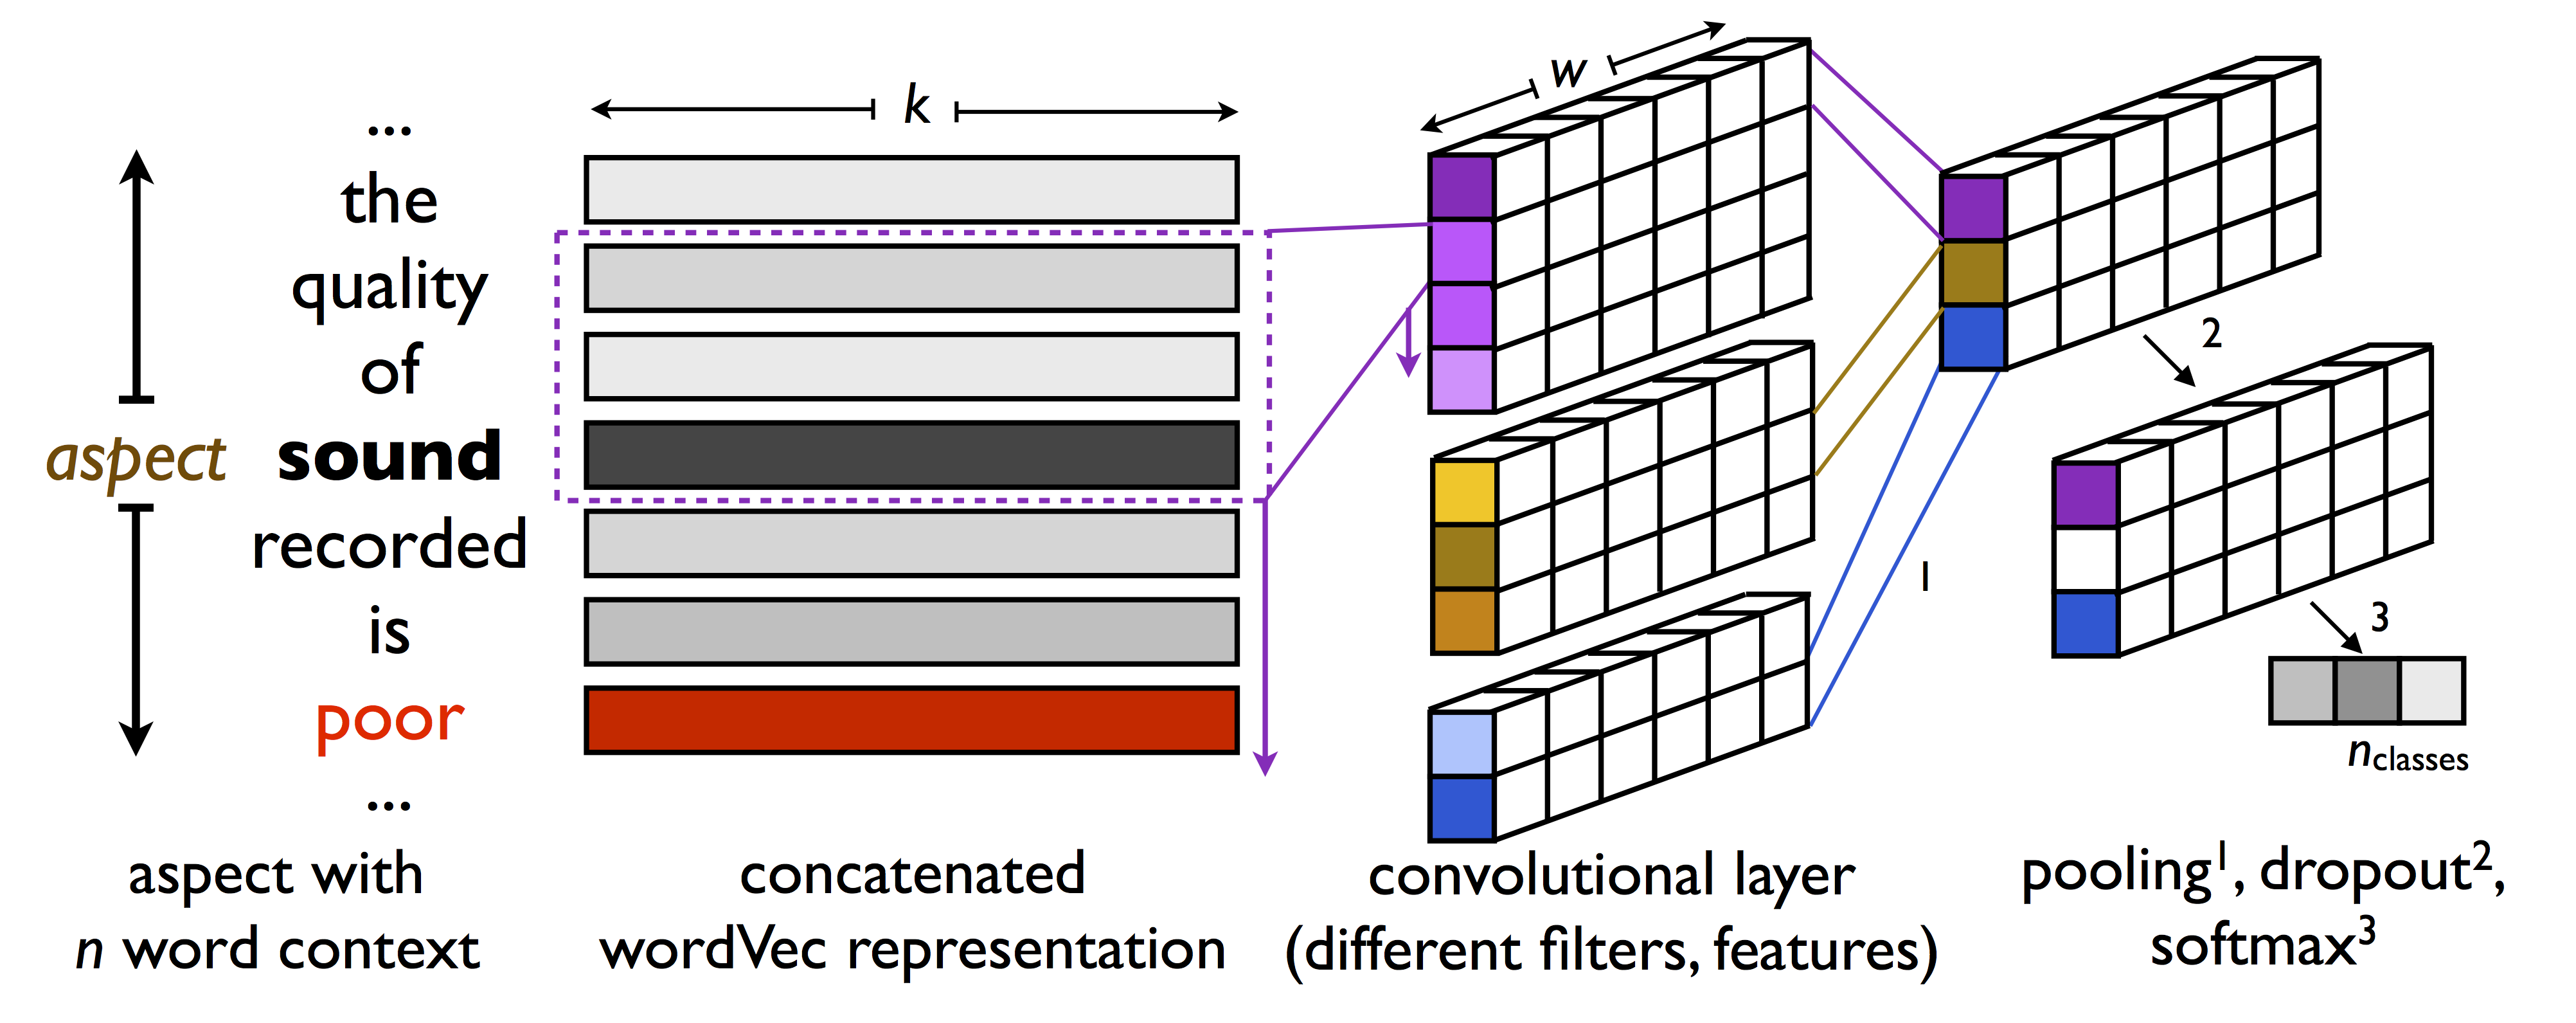
\includegraphics[width=\columnwidth]{model_architecture.png}
\end{center}
\caption{CNN Model Architecture, modeled after Kim [10]. The input is an $n$ word context, where $n$ is odd, and the center word is an identified aspect. The input is convolved with different filter sizes (3,4,5) with $w$ features. It then undergoes max-pooling (1) to pick the strongest feature.}
\label{architecture}
\end{figure}


\section{Experimental Results} 

\subsection{Aspect Discovery Model Training} 

We trained three different word2vec models. The most successful model was trained using the CBOW (continuous bag-of-words) model with a window size of 10 and feature dimension size of 300. We also ignored all words with total frequency count below 40 (this helped to remove many misspellings). We determined the performance of each model by querying the model with various aspects common to electronic products (e.g. "portability", "screen quality", etc).

\subsection{word2vec Results}

\begin{figure}[ht]
\begin{center}
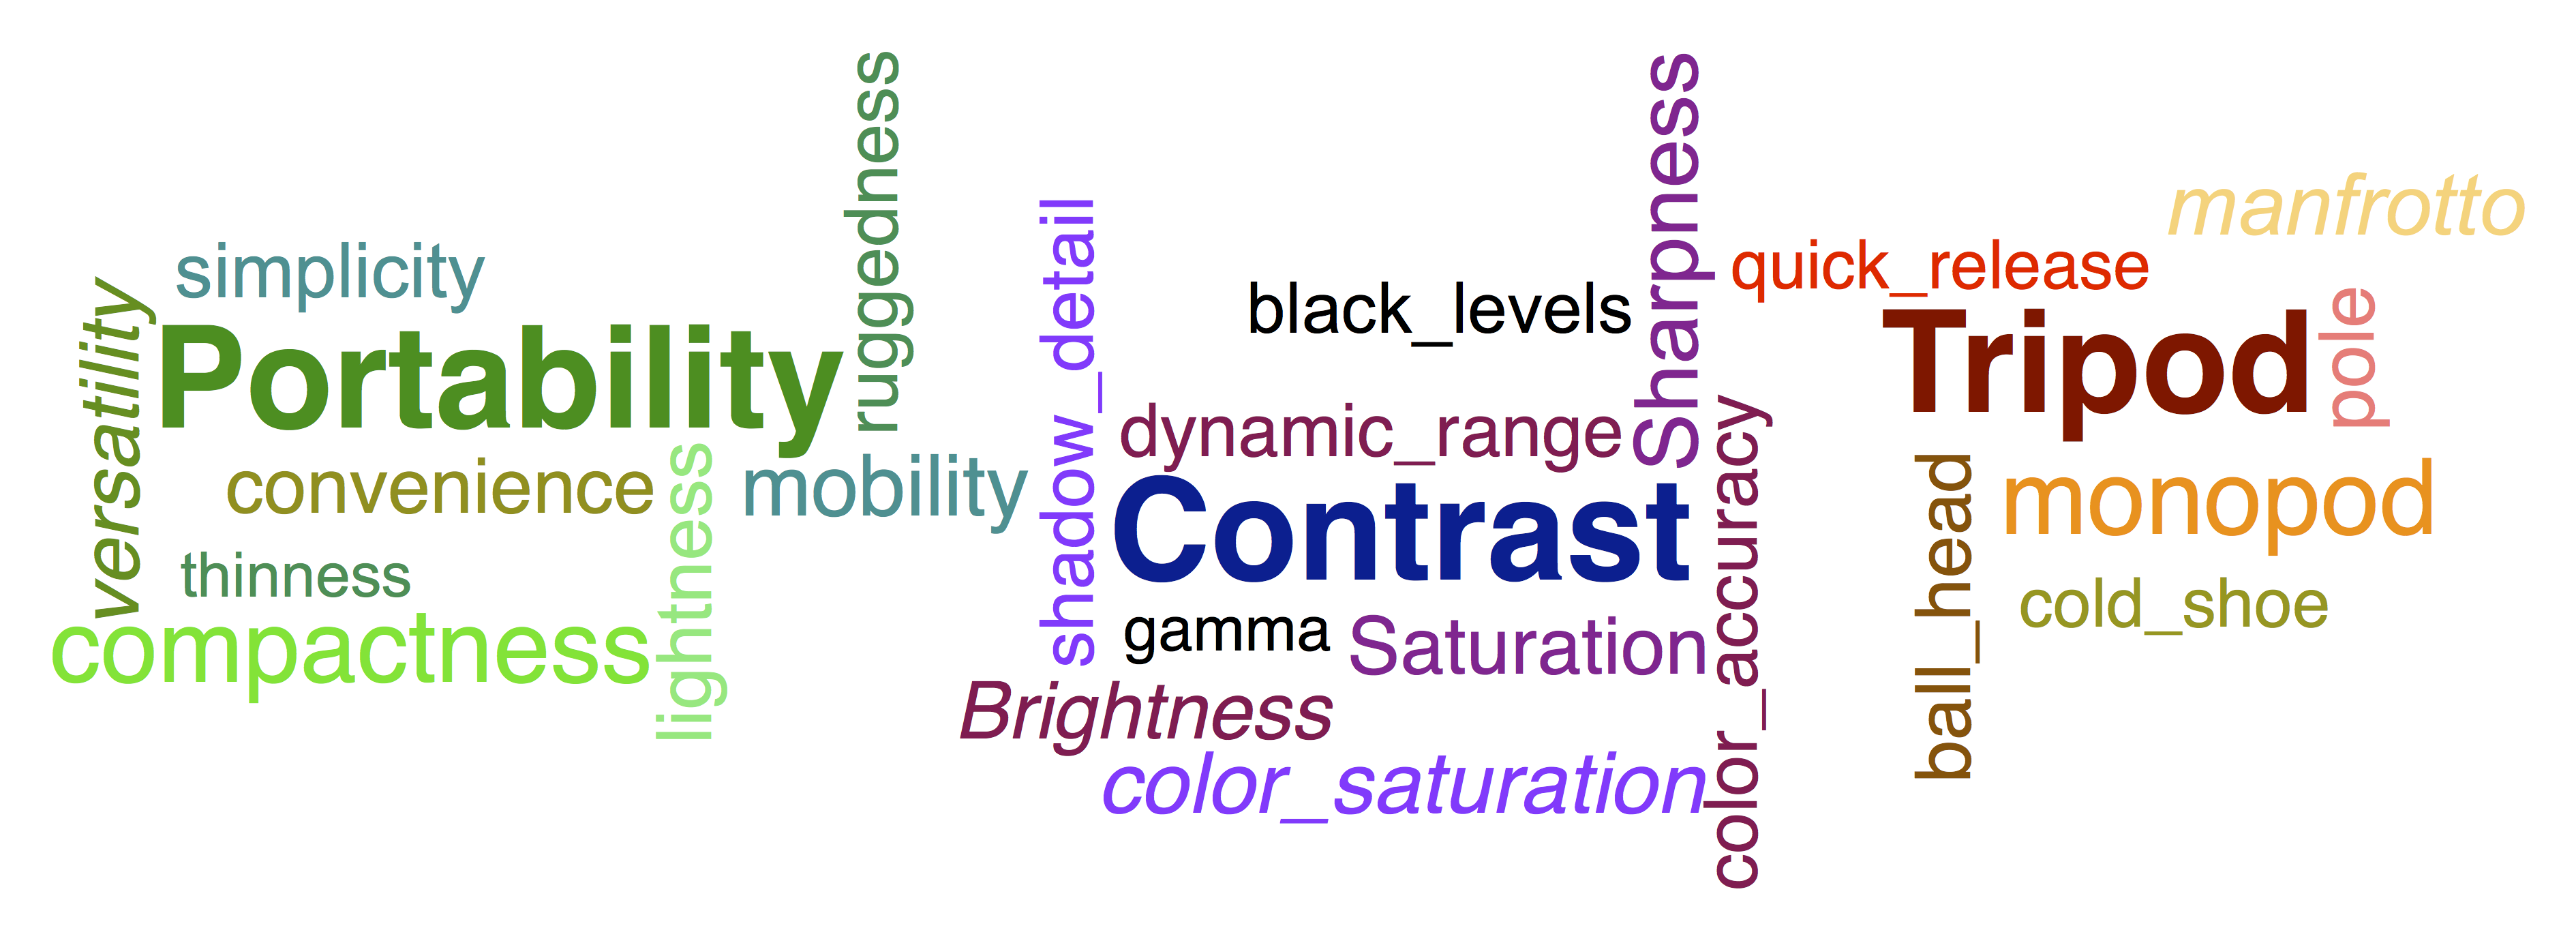
\includegraphics[width=\columnwidth]{Aspects_long.png}
\end{center}
\caption{Aspects Discovery. Word clouds generated by seeding \texttt{portability} (left), \texttt{contrast} (middle), and \texttt{tripod} (right). Words are sized according to cosine similarity with the seed word.}
\label{aspectFig}
\end{figure}

We queried our word2vec model and returned the top-$n$ results based on cosine similarity of the word vectors, as illustrated in Figure \ref{aspectFig}. After qualitative evaluation, we found that $n=5$ is a good number that maintains the quality of aspects while allowing a good discovery ratio.

As shown in Fig. \ref{aspectFig}, words like \texttt{portability} returned many synonyms as well as product aspects that are related to it (e.g. \texttt{ruggedness} and \texttt{simplicity}). Our model is also capable of returning aspects that are specific and unique to the product category it is trained on. In this case of electronic products, a query like \texttt{contrast} returned words like \texttt{shadow\_detail}, \texttt{dynamic\_range}, \texttt{black\_levels} and \texttt{gamma}, which are aspects specific to devices like monitor displays and cameras. Finally, the query \texttt{tripod} returned various aspects of camera tripods, many of them being features that are non-obvious to the layperson. For instance, \texttt{ball\_head} refers to a type of ball-shaped tripod head that allows free-pivoting along two rotational axes (as opposed to Cartesian axes), and \texttt{quick\_release} refers to tripod mounts that come with a quick-release plate. Many of these queries would otherwise perform poorly if performed on lexical databases like WordNet.


\subsubsection{ Aspect detection model }

We extracted sentences with aspects that were within our discovered aspect list, and labeled each word as either being an aspect, or not. This served as the input to a window aspect classifier with some hyperparameters FIXME, . 


\subsection{Aspect-Specific Sentiment Extraction}


% Socher's model (down the rows) vs. human labels. So there were 16 instances that human says 2 and model says 1.
%							True Labels
%			1		2		3		4		5
%1			9		16		5		10		4		44
%2			168		495		404		180		124		1371
%3			230		590		1528		488		303		3139
%4			21		70		494		490		281		1356
%5			0		0		9		65		16		90
%			428		1171		2440		1233		728		6000

As our data was entirely unlabeled, we initially attempted to bootstrap training of our CNN model using labels obtained from other trained sentiment-analysis models. We felt, however, that this would be a major limitation, as we would have labels of uncertain quality and accuracy (we discuss this more below). Hence, to properly evaluate our approach, we decided to hand label some data and use a semi-supervised approach to build a larger model. Unfortunately we did not complete our ambitious, semi-supervised goal. Below, we report our quantitative evaluation.

Using the first model developed above, we extracted 6,000 examples which consisted of an identified aspect, surrounded by a context of 5 words on either side. We padded these phrases with sentence start and end tags, and with zero vectors. Next, we hand-labeled these 6,000 examples on a 5 point scale, corresponding to Very Negative, Negative, Neutral, Positive, and Very Positive. 

We trained our CNN on this dataset, using a 10-fold cross validation strategy and reporting on a 10\% test set. The results are given in Table \ref{ModelResultsTable}. The CNN, with <hyperparameters FIXME> achieved an accuracy of FIXME on the 5 class classification, and, if we combined the classes to a coarser, 3 class (Positve, Neutral, Negative) task, achieved an accuracy of FIXME.

Next, we sought to test our original idea of ``bootstrapping" labels using existing pre-trained models. On the one hand, there are models that are trained on much larger amounts of labeled data, sometimes even down to the unigram level, e.g. Socher et al [7]. On the other hand, these models are often trained on other domains ([7] was trained on movie reviews), and it is still an open question as to the degree of cross-domain transfer. To test this, we ran the Stanford CoreNLP Sentiment Annotator [7], which also outputs 5 classes, on our 6,000 labeled examples. The 5-class accuracy was 42.3\%, while the coarser 3 class accuracy was 51.1\%.

We must be upfront and say that our point of performing this was \textbf{not} to use [7] as a baseline for comparison: indeed, it was trained out of domain, while our model was trained within domain. (Note, however, that [7] reported a test accuracy within their own dataset of 45.7\% on a 5 class task, so their performance is comparable to what we found.) Rather, we performed this analysis to gauge the upper limit on our model's reliability if it were only trained using labels obtained from out-of-domain pre-trained models (which, this analysis shows, has ~50\% accuracy with respect to a labeled gold standard on a 5 class task).

\begin{table}[t]
\begin{center}
\begin{tabular}{lll}
\multicolumn{1}{c}{\bf Aspect Detection Model}  &\multicolumn{1}{c}{\bf Recall}  \\ \hline
Sliding Window Classifier \textsuperscript{1} & 8X.X\% \textbf{(FIXME)} \\
&\\
\end{tabular}
\begin{tabular}{lll}
\multicolumn{1}{c}{\bf Sentiment Model}  &\multicolumn{1}{c}{\bf 3-class Accuracy} &\multicolumn{1}{c}{\bf 5-class Accuracy} \\ \hline
 Convolutional Neural Network \textsuperscript{1} & 79.4\% \textbf{(FIXME)} & 64\% \textbf{(FIXME)} \\
 Pre-trained out-of-domain RNTN [7]\textsuperscript{2}       & 51.1\% & 42.3\% \\
\end{tabular}
\end{center}
\caption{Performance of different models. Top: Recall of the RNN in our aspect detection model. Bottom: Accuracies on the sentiment analysis task. \textsuperscript{1} is described in Fig. \ref{architecture} and was trained in domain, while \textsuperscript{2} is an RNTN pre-trained on movie review data. The interpretation is discussed more in text.}
\label{ModelResultsTable}
\end{table}



\subsection{Qualitative evaluation of sentiment}

\textbf{Evaluation}: We will construct word cloud visualizations color coded to express sentiment. We will also perform comparisons with ``expert review" sites like CNET and DPReview (e.g. DPReview specifically rates digital cameras along certain chosen dimensions).


compare with google product reviews / cnet reviews

Error analysis (but actually we don't know if our model fails on these, we don't really have item level aspect

One common aspect that our method identified was \texttt{speed}, in terms of computer or processing speed. This also led to the discovery of \texttt{speed\_limit}, in the context of GPS reviews where GPSes are programmed with the speed limit of roads. While it might be arguable that knowing the road speed limit is a relevant aspect of a GPS, this highlighted the fact that our model might not be able to capture instances where words have different meanings in different contexts.

One problem with aspect-specific sentiment analysis in product reviews is that many reviewers discuss how the new product fares in relation to an older, similar product they owned. For example, phrases like ``my old laptop was better" seems semantically positive, but reflects negative sentiment with respect to the product being discussed. We hoped that increasing the context window would allow the model to pick up comparative words (especially that interacts with which is the subject and object of comparison).



word cloud
size = frequency of aspect over several reviews
color = valence

\section{Discussion}

Even our mediocre labeling (6000 examples) was comparable with many existing datasets out there (e.g. the Beer Advocate dataset and Camera Review dataset reported in [6] had about 8,000 and 4,000 labeled sentences respectively).

\section{Conclusion}

conclusion

cost efficient, time consuming






\subsubsection*{Acknowledgments}

We would like to acknowledge funding for computing resources provided by the Deep Social Learning Lab at Stanford.

\subsubsection*{References} % chronological. Use APA

\small{

%Word2Vec papers
[i] Mikolov, T. \& Chen, K. \& Corrado, G. \& Dean, J. (2013). Efficient Estimation of Word Representations in Vector Space. In Proceedings of Workshop at ICLR, 2013.

[ii] Mikolov, T. \& Chen, K. \& Corrado, G. \& Dean, J. (2013). Distributed Representations of Words and Phrases and their Compositionality. In Proceedings of NIPS, 2013.

[1] Titov, I., \& McDonald, R. T. (2008). A Joint Model of Text and Aspect Ratings for Sentiment Summarization. In {\it ACL} (Vol. 8, pp. 308-316).

[2] Brody, S., \& Elhadad, N. (2010). An unsupervised aspect-sentiment model for online reviews. In {\it Human Language Technologies: The 2010 Annual Conference of the North American Chapter of the Association for Computational Linguistics} (pp. 804-812). Association for Computational Linguistics.

[3] Jo, Y., \& Oh, A. H. (2011). Aspect and sentiment unification model for online review analysis. In Proceedings of the fourth ACM international conference on Web search and data mining (pp. 815-824). ACM.


[4] Engonopoulos, N., Lazaridou, A., Paliouras, G., \& Chandrinos, K. (2011). ELS: a word-level method for entity-level sentiment analysis. In {\it Proceedings of the International Conference on Web Intelligence, Mining and Semantics}


[5] Moilanen, K., \& Pulman, S. (2009). Multi-entity Sentiment Scoring. In {\it Recent Advances in NLP} (pp. 258-263).


[6] Lakkaraju, H., Socher, R, \& Manning, C. (2014). Aspect Specific Sentiment Analysis using Hierarchical Deep Learning. {\it NIPS Workshop on Deep Learning and Representation Learning}

[7] Socher, R., Perelygin, A., Wu, J. Y., Chuang, J., Manning, C. D., Ng, A. Y., \& Potts, C. (2013). Recursive deep models for semantic compositionality over a sentiment treebank. In {\it Proceedings of the conference on Empirical Methods in Natural Language Processing (EMNLP)} (Vol. 1631, p. 1642).


%[8] Ghose, A., \& Ipeirotis, P. G. (2007). Designing novel review ranking systems: predicting the usefulness and impact of reviews. In {\it Proceedings of the Ninth international conference on Electronic commerce} (pp. 303-310). ACM.

%[9] Chen, P. Y., Dhanasobhon, S., \& Smith, M. D. (2008). All reviews are not created equal: The disaggregate impact of reviews and reviewers at Amazon.com. Available at SSRN: http://ssrn.com/abstract=918083 

%[10] Dai, W., Jin, G. Z., Lee, J., \& Luca, M. (2012). Optimal aggregation of consumer ratings: an application to Yelp.com (No. w18567). National Bureau of Economic Research. 


[8] McAuley, J., Targett, C., Shi, J., \& van den Hengel, A. (2015). Image-based recommendations on styles and substitutes. {\it ACM Special Interest Group on Information Retrieval (SIGIR)}

[9] Bird, Steven, Loper, E. and Klein, E. (2009). Natural Language Processing with Python. O'Reilly Media Inc.

[10] Kim, Y. (2014). Convolutional neural networks for sentence classification. EMNLP.

%% this paper isn't that relevant. it's an evaluation system.
%[2] Ward, C. B., Choi, Y., Skiena, S., \& Xavier, E. C. (2011). Empath: A framework for evaluating entity-level sentiment analysis. In {\it Emerging Technologies for a Smarter World (CEWIT), 2011 8th International Conference \& Expo}. (pp. 1-6). IEEE.


%
%Wang, H., Lu, Y., & Zhai, C. (2010, July). Latent aspect rating analysis on review text data: a rating regression approach. In Proceedings of the 16th ACM SIGKDD international conference on Knowledge discovery and data mining (pp. 783-792). ACM.
%
%Yatani, K., Novati, M., Trusty, A., & Truong, K. N. (2011, May). Review spotlight: a user interface for summarizing user-generated reviews using adjective-noun word pairs. In Proceedings of the SIGCHI Conference on Human Factors in Computing Systems (pp. 1541-1550). ACM.



}

\end{document}
